% Compile with:
% pdflatex supplement.tex
% bibtex supplement
% pdflatex supplement.tex
% pdflatex supplement.tex
\documentclass[letterpaper]{article}
\usepackage[submission]{aaai2027}
\usepackage[hyphens]{url}
\usepackage{graphicx}
\urlstyle{rm}
\def\UrlFont{\rm}
\usepackage{natbib}
\usepackage{caption}
\frenchspacing

\usepackage{amsmath}
\usepackage{amssymb}
\usepackage{amsthm}
\usepackage{booktabs}
\usepackage{multirow}
\usepackage{placeins}
\usepackage{xcolor}

\pdfinfo{
/TemplateVersion (2027.1)
}

\newcommand{\system}{\textsc{AlgoTutorGen}}
\newcommand{\machineok}{\textsc{Machine OK}}
\newcommand{\traceir}{\textsc{SemanticTrace}}
\newcommand{\scenegraph}{\textsc{SceneGraph}}
\newcommand{\runtime}{\textsc{Web Runtime}}
\newcommand{\ssv}{\textsc{SSV}}
\newcommand{\pvcr}{\textsc{PVCR}}
\newcommand{\localresume}{\textsc{Local Resume}}
\newcommand{\globalrestart}{\textsc{Global Restart}}
\newcommand{\benchmarkname}{\textsc{AlgoTutorGen-Bench}}
\newcommand{\dbr}{\textsc{Direct-BrowserRepair (max 5)}}
\newcommand{\htmlcure}{\textsc{HTMLCure (strict)}}
\newcommand{\vtllm}{\textsc{VerifiedTrace-to-LLM-HTML}}
\makeatletter
\setlength{\@fptop}{0pt}
\setlength{\@dblfptop}{0pt}
\makeatother
\newtheorem{definition}{Definition}
\newtheorem{theorem}{Theorem}
\newtheorem{proposition}{Proposition}
\newenvironment{coltable}
  {\begin{center}\begin{minipage}{\columnwidth}\centering}
  {\end{minipage}\end{center}}
\newcommand{\promptbox}[2]{%
  \par\smallskip
  \noindent\begin{minipage}{\columnwidth}
  \colorbox{black!20}{\parbox{\dimexpr\columnwidth-2\fboxsep\relax}{\textbf{#1}}}%
  \par\nointerlineskip
  \fcolorbox{black!20}{black!3}{\parbox{\dimexpr\columnwidth-2\fboxsep-2\fboxrule\relax}{\footnotesize #2}}%
  \end{minipage}%
  \par\smallskip
}
\renewcommand{\thetable}{S\arabic{table}}
\renewcommand{\thefigure}{S\arabic{figure}}
\setcounter{secnumdepth}{0}

\begin{document}

\title{Supplementary Material: AlgoTutorGen}
\author{Anonymous Submission}
\affiliations{}
\nocopyright

\maketitle

\section{Supplement Scope and Reading Guide}

The main paper presents the complete argument and primary evidence. This document expands the executable interfaces, prompt contracts, formal derivations, measurement protocol, secondary tables, artifact provenance, and frozen English case studies. Its organization follows the two formal pipelines introduced in the paper: Semantic Synthesis and Verification (\ssv{}) produces the Verified View, and Post-Verification Creative Rendering (\pvcr{}) produces an optional Creative View.

\begin{figure*}[t]
\centering
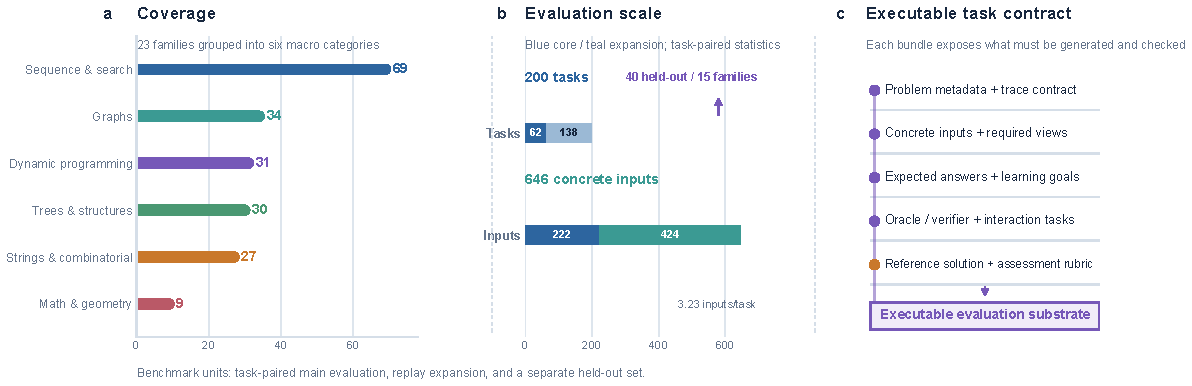
\includegraphics[width=0.94\textwidth]{figures/dataset-overview.pdf}
\caption{Complete \benchmarkname{} overview. The 200 tasks contribute one anchor input each to task-paired main comparisons and 446 additional inputs for replay-based evaluation, yielding 646 stored inputs across 23 families. Family-core contributes 62 tasks/222 inputs and expansion contributes 138/424. A separate held-out evaluation contains 40 new tasks from 15 supported families.}
\label{fig:dataset-overview-full}
\end{figure*}

\section{\machineok{} Protocol and Artifact Provenance}

\subsection{Decision Rule}

For each page, the browser harness records nine booleans: page load, visible-answer match, reachable interaction, correct feedback, wrong feedback, hint behavior, answer-reveal behavior, learning-log behavior, and protected-answer stability. A page is \machineok{} only if all nine are true. Correct and wrong feedback are tested using distinct submitted values. Hint and answer-reveal controls must change their associated pedagogical state, and the learning log must record the tested event. The ninth browser-audit check compares the protected visible-answer summary before and after the audited teaching actions. It is deliberately lighter than the independent noninterference stress suite, which compares algorithm-state, current-step, and artifact hashes after each action in 100 random sequences per page. Navigation in that stronger suite may change the step only to a verified target frame. These browser checks are offline evaluation instruments rather than fields of the online \texttt{ReleaseGate}. External requests are blocked during both audits.

\subsection{Generation and Statistical Boundaries}

The main comparison uses sample index 0 for each of 200 tasks, preventing tasks with more stored inputs from receiving greater weight. The full benchmark contains 646 samples. The primary \system{} condition uses DeepSeek-V4-Pro. Cross-model final-quality runs use DeepSeek-V4-Flash, GLM-5.2, and Kimi-K2.5: each starts from two candidates and two repair rounds, and failed tasks may receive a recorded retry with at most three candidates and three rounds. Consequently, the final cross-model table is not a uniform-call or token-matched comparison. Direct HTML receives the concrete input and expected answer and is explicitly asked to generate the complete interaction suite.

McNemar tests use paired task-level binary outcomes. Paired bootstrap confidence intervals resample tasks, not frames, actions, or individual metric checks. Holm correction applies to test families, and paired ordinal or continuous secondary scores use Wilcoxon signed-rank tests where appropriate. Frame and action totals describe implementation coverage and are not treated as independent inferential samples. A nonsignificant result is not evidence of equivalence.

\section{Formal Artifact and Release Contracts}

An input is $x=(q,i,e,c)$: algorithmic problem $q$, concrete instance $i$, optional oracle $e$, and optional reference code or strategy $c$. The model produces one instrumented solver $\widetilde S$. Executing it once under run identifier $\rho$ yields
\[
E_\rho=(y_\rho,T_\rho,Z_\rho,L_\rho),
\]
where $y_\rho$ is the final answer, $T_\rho=(e_0,\ldots,e_n)$ is the ordered typed event sequence, $Z_\rho=(z_0,\ldots,z_{n+1})$ is the sequence of per-step service snapshots, and $L_\rho=(\ell_0,\ldots,\ell_n)$ contains runtime-captured source callsites. The \ssv{} synthesis bundle is therefore $A=(\widetilde S,E_\rho,G,\bar P,R)$, comprising the instrumented solver and execution record, \scenegraph{} sequence $G$, protected pedagogical sidecar represented as the contract-checked overlay $\bar P$, and browser runtime $R$. Deterministic export produces the Verified View $W_V$. The optional \pvcr{} pipeline consumes $W_V$ and a presentation digest $D(A,x)$ and returns scoped assets $H$. If the creative contract $C_C(H,W_V)$ passes, the fixed shell exports a Creative View $W_C$; otherwise it returns $W_V$.

The online release contract is
\begin{align}
\Phi_{\mathrm{release}}(A,W,x)={}&
\Phi_{\mathrm{execution}}\land\Phi_{\mathrm{result}}
\land\Phi_{\mathrm{trace}}\notag\\
&{}\land\Phi_{\mathrm{scene}}\land\Phi_{\mathrm{runtime}},
\end{align}
where the terms check same-execution binding and callsites, available-oracle agreement, the typed event sequence and replayed service state, scene bindings, and runtime exportability. Offline evaluation additionally measures
\[
\Phi_{\mathrm{audit}}=\Phi_{\mathrm{release}}\land
\Phi_{\mathrm{feedback}}\land\Phi_{\mathrm{noninterference}}.
\]
The feedback term covers distinguishable correct and incorrect responses, hints, answer reveal, and learning-log behavior. The noninterference term requires teaching actions to preserve algorithm facts, while navigation may select another verified frame. These stronger checks are evaluation instruments rather than fields of the online \texttt{ReleaseGate}.

Direct HTML searches one open-ended artifact containing answer data, algorithm state, rendering logic, handlers, and teaching state. \system{} instead implements the refinement chain
\[
\begin{aligned}
\widetilde S&\xrightarrow{C_E}E_\rho
\xrightarrow{C_T}G\xrightarrow{C_G}R,\\
(T_\rho,G)&\xrightarrow{\mathrm{teaching}}P\xrightarrow{C_P}\bar P,\\
(G,R,\bar P)&\xrightarrow{C_B}W_V.
\end{aligned}
\]
The operational benefit comes from early rejection, reuse of verified semantic data, deterministic downstream stages, and narrower failure attribution.

\section{Executable Interfaces and Configuration}

Table~\ref{tab:stage-interfaces} states the implementation boundary of every component. The optional correctness-contract drafter remains distinct from the instrumentation layer: instrumentation binds an execution to its trace, whereas the oracle tests whether the executed algorithm is correct. The principal path begins with one instrumented solver.

\begin{table*}[t]
\centering
\small
\setlength{\tabcolsep}{3pt}
\begin{tabular}{@{}p{0.14\textwidth}p{0.17\textwidth}p{0.17\textwidth}p{0.13\textwidth}p{0.27\textwidth}@{}}
\toprule
Component & Input & Output & Construction & Blocking boundary and failure handling \\
\midrule
Instrumented-solver generation & Problem, concrete input, optional expected result, requested variants & One service-compositional solver per variant & Generated & Strict schema and function signatures; no independently authored \texttt{solve}/\texttt{trace} pair \\
Single execution and materialization & Instrumented solver and concrete input & $E_\rho$: answer, events, per-step service snapshots, and source callsites & Sandboxed execution & Common run ID; callsite and source-range checks; prefix/final replay equality; oracle agreement reported separately \\
Scene compilation & Validated \traceir{} & \scenegraph{} frames & Deterministic & One event maps to one frame; structural scene gate checks nonempty/visible objects and references \\
Teaching enrichment & Validated trace-event digest and compiled \scenegraph{} & Teaching/interaction overlay applied to the compiled scene & Generated & Strict overlay schema and sanitization; primary 30-event context retries with three events; failure remains a warning \\
\ssv{} export and runtime & Artifact, scene, sanitized teaching & Verified View and sidecar JSON & Deterministic & Online structural release gate; external-resource, nine-check browser, and noninterference tests are reported offline \\
\pvcr{} & Verified artifact/frame context & Scoped stage CSS/template/renderer & Generated & Presentation sanitizer plus browser/layout gate; rejection falls back to the Verified View; supplied nested context is not a deep-frozen security boundary \\
\bottomrule
\end{tabular}
\caption{Executable component interfaces. ``Generated'' denotes an open-ended model output; ``deterministic'' denotes project code operating on validated data.}
\label{tab:stage-interfaces}
\end{table*}

\ssv{} ends at the release of the Verified View. \pvcr{} is an optional downstream presentation pipeline: it consumes a verified artifact, operates inside the fixed tutor shell, and is omitted from the preservation and noninterference premises. Its accepted output is called the Creative View; any creative-generation, sanitizer, browser, or layout failure returns the Verified View.

\begin{table*}[t]
\centering
\small
\setlength{\tabcolsep}{3pt}
\begin{tabular}{@{}p{0.17\textwidth}p{0.14\textwidth}p{0.17\textwidth}p{0.15\textwidth}p{0.25\textwidth}@{}}
\toprule
Condition & Model & Candidate/repair policy & Runtime limits & Important boundary \\
\midrule
\system{} main & DeepSeek-V4-Pro & 2 solution variants; 2 candidates; 2 repair rounds per candidate & 32,768 output tokens; 900 s API timeout; 3,000 s task timeout; concurrency 8 & Strict warnings; teaching enabled; sample index 0 \\
Direct HTML main & DeepSeek-V4-Pro & 1 candidate; at most 2 repairs & 32,768 output tokens; 2,400 s task timeout; concurrency 8 & Expected result visible; no browser-feedback repair; self-contained HTML requested \\
Cross-model \system{} & Flash, GLM, Kimi & Initial $2\times2$; failed tasks eligible for final-quality retry up to $3\times3$ & Browser audit sharded 16 ways & Final frozen pages reported; calls/tokens differ from Direct \\
Held-out \system{} & DeepSeek-V4-Pro & 2 candidates; 2 repair rounds & 900 s API timeout; 2,400 s task timeout; concurrency 8 & Forty new tasks from 15 families \\
WebGen-Agent & DeepSeek-V4-Pro & At most 5 agent iterations & Same final browser audit & Task-adapted external code path; not a reproduction of its original benchmark \\
\htmlcure{} & DeepSeek repair; Gemini evaluator & 1 repair iteration & External requests blocked in final audit & Operates on frozen Direct pages; self-containment is part of strict failure \\
\dbr{} & DeepSeek-V4-Pro & Adaptive maximum budgets 0/1/2/3/5; early stop; best-so-far & 32,768 output tokens; 1,800 s API timeout; concurrency 32 & Same 200 hash-verified initial pages; full previous HTML; generic browser feedback \\
\bottomrule
\end{tabular}
\caption{Recorded generation and execution configuration. Counts are maximum policy budgets, not a claim that every task consumed the maximum.}
\label{tab:generation-config}
\end{table*}

JSON generation uses temperature 0.2 and text generation uses 0.3, except Kimi models, for which the provider-required value is 1.0. The API client allows four JSON-parse retries and two transport retries by default; these calls are included in logged model-call metadata when present. Remote model versions can drift.

\subsection{Sandbox and Threat Model}

Generated instrumented solvers and optional verifier functions are parsed with an AST check, executed in a separate Python child process, and receive a restricted builtin namespace plus allowlisted standard-library modules. Each function has a 30-second execution timeout, and a trace event whose serialized state exceeds 20,000 characters is rejected. The instrumentation layer binds each service event to the executing frame or AST source map and assigns the run identifier; these fields are not accepted from model output. The DSL guard rejects undocumented object methods before execution and protects service-owned visible state from direct mutation. This boundary is intended to contain accidental model-generated code and enforce the artifact contract; it is not an operating-system or container security claim against a determined adversary.

\section{Service-Compositional Trace Interface}

\subsection{Catalog and Emission Semantics}

The \texttt{TraceSession} catalog contains 21 factories. They are grouped below by the state role they expose to the trace program; grouping is descriptive and does not determine which algorithm families may use a service.

\begin{table*}[t]
\centering
\small
\setlength{\tabcolsep}{4pt}
\begin{tabular}{@{}p{0.18\textwidth}p{0.72\textwidth}@{}}
\toprule
State role & Service factories \\
\midrule
Indexed and tabular & \texttt{array}, \texttt{string}, \texttt{table}, \texttt{intervals}, \texttt{points} \\
Scalar and associative & \texttt{scalar}, \texttt{map}, \texttt{counter}, \texttt{pointer} \\
Ordered containers & \texttt{heap}, \texttt{stack}, \texttt{queue}, \texttt{deque} \\
Linked and hierarchical & \texttt{linked\_list}, \texttt{trie}, \texttt{tree}, \texttt{union\_find} \\
Graph and range structures & \texttt{graph}, \texttt{flow\_network}, \texttt{fenwick}, \texttt{segment\_tree} \\
\bottomrule
\end{tabular}
\caption{The current service catalog. The generation interface exposes service capabilities rather than a selector over algorithm-family templates.}
\label{tab:service-catalog}
\end{table*}

A supported service operation has two atomic effects:
\[
(z_t,o_t)\longmapsto(z_{t+1},e_t).
\]
It updates the represented service state and emits a typed event with stable object references, before/after values, run identifier, and automatically captured callsite. For example, \texttt{arr[i] = value}, \texttt{heap.push(x)}, \texttt{ptr.move(j)}, and \texttt{dist[node] = d} emit the corresponding set, container, pointer, or map event. Ordinary Python control flow and local variables may compute temporary values, but any canonical fact claimed by the released tutor must be introduced through a service or explicit checked semantic event. The final answer is committed by this same execution. The DSL guard statically tracks variables constructed by these factories and rejects undocumented methods and visible-state bypasses before or during sandbox execution.

\begin{table*}[t]
\centering
\small
\begin{tabular}{@{}p{0.25\textwidth}p{0.33\textwidth}p{0.32\textwidth}@{}}
\toprule
Case & Observed service composition & Family-independent state roles \\
\midrule
Coin change & \texttt{array} & Denominations and evolving values \\
Dijkstra shortest path & \texttt{graph + heap + map} & Topology, frontier priority, tentative distances \\
Permutations & \texttt{array + tree} & Candidate sequence and recursive call structure \\
Number of provinces & \texttt{array + graph + scalar + table + tree + union\_find} & Input matrix, components, counters, recursive and disjoint-set views \\
\bottomrule
\end{tabular}
\caption{Representative service compositions recovered from the saved qualitative program source.}
\label{tab:service-examples}
\end{table*}

\subsection{Full-200 Execution Trace Audit}
\label{sec:single-execution-audit}

The confirmatory audit evaluates the primary selected-final system. Its
unit of evidence is $(\text{task},\text{variant},\text{input},\rho)$,
not merely a task. All 200 tasks retain two accepted variants, giving
400 variant programs. Running both variants on every stored task input
gives $2\times646=1{,}292$ instrumented executions. Event- and
prefix-sensitive checks are aggregated strictly at the run level: a
run passes only if every applicable event or replay prefix passes.

Same-execution binding is established at record construction: the
runtime issues $\rho$ and attaches it to the answer commitment, events,
and snapshots. The audit does not accept a post-hoc pass that merely
copies one string into otherwise independent outputs. Callsite
validation checks both source range and the frozen source hash; a forged
but in-range line therefore remains invalid. Prefix replay starts from
the independently stored initial service state and applies event
transitions without executing the generated solver. This establishes
logging consistency for service-mediated state. Oracle agreement
independently evaluates whether the traced answer matches the expected
result.

The visible-state closure audit combines the service ownership rule
with end-of-step canonical digests. Ordinary local variables are
allowed and are outside the claim. A value becomes protected when it is
exported as a canonical page fact; direct mutation of such state without
a corresponding service operation is rejected. Deterministic replay is
performed in a fresh process with fixed source and input hashes, random
seed, and environment manifest. Equality is computed over canonical
answer, event, and state digests rather than run IDs or timestamps.

\begin{table*}[t]
\centering
\small
\setlength{\tabcolsep}{5pt}
\begin{tabular}{@{}p{0.25\textwidth}p{0.19\textwidth}p{0.43\textwidth}@{}}
\toprule
Check & Full-200 result & Interpretation \\
\midrule
Same-execution binding & 1,292/1,292 runs & Answer, events, and snapshots share one runtime-issued $\rho$ \\
Runtime callsite coverage & 1,292/1,292 runs & Every event in every passing run carries a non-model-authored runtime callsite \\
Source-range validity & 1,292/1,292 runs & Every callsite in every passing run resolves under the frozen source hash \\
Prefix replay equality & 1,292/1,292 runs & Every independently replayed prefix matches its recorded service state \\
Final-state equality & 1,292/1,292 runs & Replay-final and execution-final state digests agree \\
Oracle agreement & 1,292/1,292 runs & Instrumented answers agree with the trusted expected results \\
Unlogged visible mutation & 0/1,292 runs & No protected canonical fact changes without a service event \\
Deterministic replay & 1,292/1,292 runs & Fresh-process canonical answer, event, and state digests agree \\
\bottomrule
\end{tabular}
\caption{Observed results of the Full-200 execution audit over 200 tasks, 400 accepted variant programs, and 1,292 instrumented executions obtained by running two variants on each of 646 stored task inputs. Event- and prefix-sensitive rows count a run as passing only when all of its events or prefixes pass.}
\label{tab:single-execution-results}
\end{table*}

All eight prespecified checks pass. The result establishes that the
accepted answer, event sequence, per-step service snapshots, runtime-captured source callsites,
and replayed states are mutually bound to one instrumented execution
for every tested run. Oracle agreement is reported separately from
replay equality because it evaluates the final algorithmic result,
whereas the other rows evaluate the integrity of the execution record.

\subsection{Negative Fault Injection}

For each accepted run, the injector selects one applicable site for
each fault family: deleting a state-changing event, swapping an
order-sensitive adjacent pair, changing a before/after value, changing
a canonical snapshot, changing the final answer, forging a callsite, or
bypassing a service to mutate protected visible state. Each mutation is
revalidated from a fresh copy of the accepted record. This produces
1,292 injected cases per family and 9,044 negative cases in total.
Deletions of explanation-only events and swaps of commutative
operations are not selected, because they need not change canonical
semantics. One semantics-preserving reserialization control is also
evaluated for every accepted run.

\begin{table*}[t]
\centering
\small
\begin{tabular}{@{}p{0.25\textwidth}p{0.47\textwidth}p{0.16\textwidth}@{}}
\toprule
Injected fault & Expected detection path & Observed outcome \\
\midrule
Delete state-changing event & Prefix or final replay mismatch & 1,292/1,292 rejected \\
Swap order-sensitive events & Prefix replay, dependency, or before-state mismatch & 1,292/1,292 rejected \\
Modify before/after & Atomic-transition validation or replay mismatch & 1,292/1,292 rejected \\
Modify canonical state & Snapshot/replay digest mismatch & 1,292/1,292 rejected \\
Modify final answer & Same-run answer commitment, final event, or oracle mismatch & 1,292/1,292 rejected \\
Forge source line & Runtime callsite/source-hash binding failure & 1,292/1,292 rejected \\
Bypass a service mutation & Visible-state closure or end-of-step digest mismatch & 1,292/1,292 rejected \\
\midrule
All negative injections & Any applicable validator path above & 9,044/9,044 rejected \\
Semantics-preserving control & Canonical answer, event, and state digests remain equal & 1,292/1,292 accepted \\
\bottomrule
\end{tabular}
\caption{Negative fault-injection results for the execution-record validator. One applicable mutation from each family is injected into every accepted run. A paired semantics-preserving control rules out a trivial reject-all validator.}
\label{tab:single-execution-mutations}
\end{table*}

All case-level and aggregate outputs are stored in
\path{single_execution_trace_audit.json}. The top-level record includes
\texttt{schema\_version}, source commit and source hash, environment
manifest, and scope counts for tasks, variants, inputs, runs, and
events. Each case stores stable task, variant, and input identifiers,
$\rho$, source hash, answer and state digests, event count, the eight
check outcomes, oracle details, and mutation outcomes. The aggregate
section reports numerators and denominators rather than only rounded
percentages.

Every applicable corruption in the seven fault families is rejected,
while all semantics-preserving controls are accepted. This paired
positive/negative design rules out a validator that passes untouched
records without checking them or rejects every modified record
indiscriminately. Together with Table~\ref{tab:single-execution-results},
the result establishes mechanical fidelity to the instrumented
execution.

\subsection{Wrong-but-Self-Consistent Solver Audit}

Beyond record-level corruptions, we mutate solvers before execution to
construct 60 wrong-but-self-consistent runs across 30 tasks spanning all
23 algorithm families. All 60 pass internal replay-consistency checks,
yet the oracle-backed pipeline detects every result mismatch and the
release gate rejects every case, yielding zero erroneous releases and
demonstrating independent semantic assurance before release.

\subsection{Blinded Dual-Reviewer Source-to-Trace Audit}
\label{sec:human-trace-audit}

We therefore evaluate algorithmic validity separately. Two reviewers
from the research team with algorithms and data-structures training label 120
complete traces from 60 stratified tasks spanning all 23 families. Both
generated variants are audited for every sampled task, yielding 3,883
event judgments. The blinded review interface shows the problem,
concrete input, expected output, complete source with stable line
numbers, ordered events, source references, pre-state, operation,
post-state, explanation, and final output. Method identity, automatic
gate outcomes, and the other reviewer's labels are hidden. Original
labels produced independently under this blinding are retained for
agreement statistics; disagreements and disputed algorithmic
interpretations receive a separate technical review.

\begin{table*}[t]
\centering
\small
\setlength{\tabcolsep}{5pt}
\begin{tabular}{@{}p{0.29\textwidth}p{0.22\textwidth}p{0.37\textwidth}@{}}
\toprule
Human-audit measure & Result & Interval or interpretation \\
\midrule
Trace-perfect task & 59/60 (98.3\%) & Wilson 95\% CI [91.1, 99.7] \\
Critical-error task & 0/60 (0.0\%) & One-sided 95\% upper bound 4.9\% \\
Trace-perfect variant & 119/120 (99.2\%) & Descriptive variant-level result \\
Critical-error variant & 0/120 (0.0\%) & No confirmed critical semantic error \\
Source exact or adjacent & 3,878/3,880 (99.95\%) & Strict line-proximity measure \\
Source non-adjacent but aligned & 2/3,880 (0.05\%) & Same logical statement block \\
Incorrect source attribution & 0/3,880 (0.0\%) & No confirmed source-attribution error \\
Source unverifiable & 3/3,883 (0.08\%) & Excluded from the source-alignment denominator \\
State transition correct & 3,883/3,883 (100.0\%) & Final technically reviewed labels \\
Algorithmic operation correct & 3,883/3,883 (100.0\%) & Final technically reviewed labels \\
Explanation consistent & 3,882/3,883 (99.97\%) & One noncritical inconsistency in one variant \\
Trace-perfect agreement & Cohen's $\kappa=1.000$ & Gate specified before labeling passed \\
Critical-error agreement & Cohen's $\kappa=1.000$ & Gate specified before labeling passed \\
\bottomrule
\end{tabular}
\caption{Blinded dual-reviewer source-to-trace audit of source alignment, state-transition and operation correctness, and explanation consistency. The task is the primary statistical unit; a task is trace-perfect only when both generated variants are trace-perfect. Agreement uses the original independently produced labels, whereas correctness results use the final technically reviewed labels.}
\label{tab:human-trace-audit}
\end{table*}

The audit finds no confirmed critical semantic error. A disputed
dynamic-programming event initially flagged as an incorrect transition
is confirmed by technical review to match the source and recurrence,
and is corrected before computing the final outcome. The one remaining
non-perfect task contains a single noncritical explanation inconsistency
in one variant under the final labels. Among the 3,880 source-verifiable
events, two point to non-adjacent lines in the same logical statement
block and remain semantically aligned; no event has an incorrect source
attribution. The three source-unverifiable events are excluded from the
source-alignment denominator and do not by themselves fail trace-perfect
status. No reviewed event contains an incorrect state transition or
algorithmic operation.

The human-audit gates specified before labeling require a task-perfect Wilson lower
bound of at least 90\%, a critical-error one-sided upper bound of at
most 5\%, a source-alignment lower bound of at least 90\%, and Cohen's
$\kappa\geq0.60$ for the key judgments. The observed values are 91.1\%,
4.9\%, 99.95\%, and 1.000, respectively. All four gates pass, and the
outcome specified before labeling is \textsc{Pass}. We therefore report high
sampled algorithmic trace validity and a low critical-error bound.

\FloatBarrier

\subsection{Full-200 Atomic-Service and Separated-Trace Ablation}
\label{sec:atomic-service-ablation}

To isolate atomic state/event ownership, we run a separate paired
Full-200 ablation under the same tasks, DeepSeek-V4-Pro model,
generation policy, validators, compiler, and fixed shell. Atomic-service
uses \textsc{TraceSession} operations that jointly mutate represented
state and emit events. The ALGOGEN-style separated-trace condition
maintains algorithm state in ordinary Python variables, requires the
model to emit the corresponding event claim separately after a state
change, and provides no helper that binds the two operations. It retains
the same downstream pipeline and therefore serves as an interface-level
matched control rather than a reimplementation of ALGOGEN's VTA/RSL
renderer.

\begin{table*}[t]
\centering
\scriptsize
\setlength{\tabcolsep}{3.5pt}
\begin{tabular}{@{}lrrrrl@{}}
\toprule
Measure & Atomic-service & Separated-trace & Difference & 95\% CI & Paired test \\
\midrule
\machineok{} & 183/200 & 162/200 & $+10.50$ pp & [$3.50,17.00$] pp & McNemar $p=.00460$ \\
Generation pass & 187/200 & 164/200 & $+11.50$ pp & [$5.00,18.00$] pp & McNemar $p=.00109$ \\
Model calls/task & 6.235 & 7.025 & $-0.790$ & [$-1.540,-0.025$] & -- \\
Repair calls/task & 1.000 & 1.880 & $-0.880$ & [$-1.130,-0.630$] & -- \\
Tokens/task & 85{,}189.8 & 94{,}081.2 & $-8{,}891.3$ & [$-19{,}072.0,1{,}526.9$] & -- \\
API latency/task & 615.7 s & 698.6 s & $-82.8$ s & [$-155.9,-8.5$] s & -- \\
End-to-end time/task & 619.6 s & 704.1 s & $-84.5$ s & [$-158.0,-9.8$] s & -- \\
\bottomrule
\end{tabular}
\caption{Paired Full-200 atomic-service ablation. The separated-trace
condition is an ALGOGEN-style state/event interface under the same
downstream tutor stack. Differences are Atomic-service minus
Separated-trace. Confidence intervals use 10,000
task-level paired-bootstrap resamples; binary outcomes additionally use
exact two-sided McNemar tests.}
\label{tab:atomic-service-ablation}
\end{table*}

The \machineok{} discordant pairs are 36 Atomic-service-only and 15
Separated-trace-only; generation-pass discordances are 35 and 12. After
excluding the 23 pilot cases, the remaining 177 pairs retain the same
direction: \machineok{} is 164/177 versus 142/177 (\(+12.43\) points;
95\% CI [5.65, 19.77]; McNemar \(p=.00126\)), and generation pass is
168/177 versus 144/177 (\(+13.56\) points; 95\% CI [6.78, 20.34];
\(p=.000182\)).

Atomic-service and Separated-trace produce auditable execution records
for 187 and 164 tasks, respectively, with 152 paired records observable
in both conditions. All 152 pairs pass execution validation,
same-execution binding, prefix replay, absence of unlogged mutations,
and state/event agreement in both arms. Atomic ownership therefore raises
the yield of valid auditable records while preserving the same
validation standard. Observed Separated-trace generation failures
include nine claim mismatches, five missing pending state transitions,
and one unlogged transition, matching the coordination burden removed by
atomic service operations.

\FloatBarrier

\subsection{Full-200 Service Reuse and Prompt-Guidance Ablation}
\label{sec:service-ablation}

We evaluate service reuse on a separate frozen Full-200 artifact set
rather than pooling it with the 400-variant, 1,292-run execution
audit. The service audit contains 200 tasks, 399 accepted variants, and
23 algorithm families; one task retains only one accepted variant.
Twenty of the 21 catalog services appear, \texttt{intervals} is unused,
and no out-of-catalog \texttt{TraceSession} factory call is observed.
At least two services are composed in 187/200 tasks (93.5\%) and
297/399 variants (74.44\%). Fifteen services recur across at least two
algorithm families, and 13 recur across at least two broader analysis
groups. The most widely reused service, \texttt{array}, appears in 138
tasks and 18 families.

The paired prompt ablation uses the same 200 tasks, inputs,
DeepSeek-V4-Pro model, temperature, candidate and repair budgets, token
limit, timeout, and exposed oracle. The hybrid condition retains the
service API, output schema, family templates, and task strategy
guidance. The service-only condition preserves the service API, schema,
and neutral composition examples but removes the family templates and
strategy guidance. Differences below are Service-only minus Hybrid;
bootstrap intervals use 10,000 task-level resamples.
All paired results use frozen Full-200 outcomes under the same Hybrid
and Service-only conditions.

\begin{table*}[t]
\centering
\small
\setlength{\tabcolsep}{4pt}
\begin{tabular}{@{}p{0.25\textwidth}p{0.15\textwidth}p{0.15\textwidth}p{0.16\textwidth}p{0.16\textwidth}@{}}
\toprule
Measure & Hybrid & Service-only & Difference (pp) & 95\% CI / decision \\
\midrule
First specification valid & 121/200 & 85/200 & $-18.0$ & [$-27.0,-9.0$]; Holm $p=.000471$ \\
Final generation pass & 200/200 & 181/200 & $-9.5$ & [$-14.0,-5.5$]; Holm $p=.0000572$ \\
\machineok{} & 198/200 & 181/200 & $-8.5$ & [$-12.5,-4.5$]; noninferiority failed \\
Unknown-DSL-call-free & 194/200 & 171/200 & $-11.5$ & [$-17.0,-6.5$]; Holm $p=.000238$ \\
\bottomrule
\end{tabular}
\caption{Prompt-matched Full-200 ablation. Service-only produces 181 \machineok{} tutors versus 198 for Hybrid and does not meet the prespecified $-3$-percentage-point noninferiority boundary.}
\label{tab:service-prompt-ablation}
\end{table*}

The results support broad service reuse while
showing that the current family and strategy guidance remains
operationally useful.

\section{Relation to ALGOGEN's VTA and RSL}

ALGOGEN and \system{} share the premise that execution state should be separated from deterministic rendering, but they use different generation abstractions and target different released artifacts~\cite{liaokunpeng-etal-2026-algogen}. ALGOGEN's VTA-JSON defines a shared many-sorted operation core; its tracker instructions additionally specify graph-, dynamic-programming-, sorting-, and other family requirements, and RSL generation consumes algorithm-family context. \system{} moves the generation boundary to service operations and adds a fixed interactive-teaching shell. The Full-200 separated-trace arm imports this shared state/event separation into the same tutor compiler and shell, making the interface contribution experimentally identifiable without conflating released modalities. Table~\ref{tab:algogen-comparison} states this distinction without treating the two systems as directly comparable on one performance number.

\begin{table*}[t]
\centering
\footnotesize
\setlength{\tabcolsep}{3pt}
\begin{tabular}{@{}p{0.16\textwidth}p{0.37\textwidth}p{0.37\textwidth}@{}}
\toprule
Dimension & ALGOGEN & \system{} \\
\midrule
Released artifact & Algorithm visualization rendered to video, figure, or interactive backend & Self-contained interactive tutor with trace, controls, feedback, hints, answer reveal, and learning log \\
Generated trace interface & Executable tracker emits VTA-JSON operations & Python control flow composes \texttt{TraceSession} service objects that emit \traceir{} events \\
Conditioning unit & Shared VTA core plus view-specific and algorithm-family guidelines & Service capabilities and their composition; no family label enters the service factory interface \\
State/visual update & Algorithm-state update and VTA visualization operation are separately authored & Supported service mutation and semantic-event emission are coupled for represented state \\
Rendering control & Deterministic renderer controlled by RSL, including family context & Deterministic \traceir{}--\scenegraph{}--browser path; optional compiler hints remain outside the generation interface \\
Pedagogy and interaction & Not the central artifact contract & Fixed shell owns code, timeline, teaching, interaction, feedback, log, and answer \\
Creative presentation & RSL specializes style before backend rendering & Optional \pvcr{} runs after semantic release and owns only the central stage slot \\
Failure boundary & Tracker, VTA schema/semantics, RSL, and backend rendering & Specification, service/trace, scene, teaching, runtime, and optional presentation boundaries \\
Scope limitation & Family-conditioned guidance remains part of the published workflow & The current prompt retains high-frequency family recipes and one benchmark-specific clarification; compiler hints also remain, so only the generated service interface is claimed to be family-agnostic \\
\bottomrule
\end{tabular}
\caption{Design-space comparison between ALGOGEN and \system{}. The target modalities differ, so the table describes interfaces and ownership rather than asserting a direct performance ranking.}
\label{tab:algogen-comparison}
\end{table*}

\section{Prompt Engineering}

Table~\ref{tab:prompt-modules} presents the prompts by role before giving representative instructions, following a module-first organization. Dynamic user messages are assembled from the concrete problem, input, expected output when exposed by the protocol, verified execution-record digest, or a structured failure report. The anonymous artifact must bundle the exact instrumented-solver and repair prompts used for the confirmatory run. Some production prompts are Chinese; the English boxes below preserve their operational structure and constraints but are not byte-identical transcripts.

\begin{table*}[t]
\centering
\small
\setlength{\tabcolsep}{3pt}
\begin{tabular}{@{}p{0.15\textwidth}p{0.17\textwidth}p{0.16\textwidth}p{0.25\textwidth}p{0.17\textwidth}@{}}
\toprule
Module & Context & Required output & Hard boundary & Retry trigger \\
\midrule
Executable spec & Problem, input, optional expected, requested variants & Strict instrumented-solver JSON & Fixed fields; one executable per variant; documented \texttt{TraceSession} DSL; no model-authored run ID/callsite; no HTML/rendering & JSON parse, schema, sandbox, execution-record, replay, oracle, or release failure \\
Optional correctness contract & Problem, input, optional expected & \path{correctness-contract-v1} JSON & Expected has priority; oracle returns answer and is not a proof & Schema/oracle failure \\
Spec repair & Previous complete JSON plus structured diagnostics & Complete replacement instrumented-solver JSON & Minimal targeted change; preserve signatures and DSL; no invented methods or manually supplied callsites & Bounded round while candidate remains \\
Teaching overlay & Digest of verified frames & \texttt{step}, \texttt{teaching}, \texttt{interaction} only & Read-only algorithm facts; checkpoint answer must follow from supplied frame & Parse/schema failure; retry with three frames \\
\pvcr{} generation & Verified artifact and current frame context & Scoped style/template/render function & Presentation-only generation contract; sanitizer checks required scripts and stable IDs & Browser/layout failure; fallback to Verified View \\
\pvcr{} repair & Previous creative assets, verified digest, structured overlap/clipping report & Replacement scoped creative assets & Repair presentation only; preserve shell IDs, trace, state, and result & One bounded repair before Verified View fallback \\
Direct HTML baseline & Same task/input/expected and teaching requirements & Complete self-contained HTML & No private contract claim; all page behavior generated together & Whole-page structured repair \\
Screenshot judge & Screenshot and rubric & Strict score JSON & Visible evidence only; no correctness or release decision & Parse retry only \\
\bottomrule
\end{tabular}
\caption{Prompt modules and hard boundaries.}
\label{tab:prompt-modules}
\end{table*}

\subsection{Representative English Prompt Skeletons}

\promptbox{System Prompt: SSV Executable Specification}{
\textbf{Role:} Generate one executable instrumented solver per requested variant. Do not generate independent \texttt{solve(input\_data)} and \texttt{trace(input\_data)} functions.\\
\textbf{Return:} One strict JSON object containing \texttt{problem\_title}, \texttt{input\_contract}, optional \texttt{verifier\_code}, and one or more \texttt{variants}.\\
\textbf{Execution contract:} Use ordinary Python control flow over documented \texttt{TraceSession} factories and methods. The same execution must compute the final answer and produce all visible per-step service snapshots and events.\\
\textbf{Checks:} Every canonical page fact must originate from service state or an explicit checked event; every value must be JSON serializable; the runtime supplies the run ID and callsite.\\
\textbf{Forbidden:} A second answer-producing function; model-authored \texttt{code\_line}; direct writes to protected visible state; HTML, CSS, JavaScript, renderer fields, project imports, undocumented DSL methods, or extra schema keys.
}

\promptbox{System Prompt: SSV Targeted Repair}{
\textbf{Context:} Original request, previous complete specification, and typed schema, sandbox, answer-agreement, state-size, or release diagnostics.\\
\textbf{Instruction:} Return a complete replacement JSON object, but make the smallest correction that resolves the reported boundary. Preserve variant count, function signatures, and DSL style.\\
\textbf{Failure localization:} Schema errors change structure; Python exceptions change the indicated code path; replay mismatches repair the corresponding service-mediated transition; oracle disagreement repairs the algorithm rather than rewriting trace metadata; oversized events retain only visualization-relevant state.\\
\textbf{Forbidden:} Splitting the solution into independent solver and tracer functions, manually filling callsites, bypassing services for visible state, or inventing object methods.
}

\promptbox{System Prompt: Read-Only Teaching Enrichment}{
\textbf{Source of truth:} A digest of selected, validated \traceir{} frames, including operation, targets, dependencies, before/after values, state diff, adjacent-step summaries, and code line.\\
\textbf{Return:} \texttt{frames[step, teaching, interaction]} only. Teaching may contain \texttt{what}, \texttt{why}, formula, invariant, common mistake, and hint; interaction may contain one grounded prediction checkpoint.\\
\textbf{Grounding rule:} The answer and feedback must follow from the supplied frame.\\
\textbf{Forbidden:} Changing operation, targets, dependencies, state, result, event order, or code line.
}

\promptbox{System Prompt: Post-Verification Creative Rendering}{
\textbf{Read-only context:} Problem description, concrete input, verified result, release summary, state-key summary, and selected verified frames.\\
\textbf{Return:} Only \texttt{<style id="creative-stage-style">}, an optional stage template, and a script defining \texttt{window.renderCreativeStage(ctx)}.\\
\textbf{Scope:} Draw the problem-specific main stage inside the deterministic shell; all frame changes must read \texttt{ctx.frame}, \texttt{ctx.state}, and \texttt{ctx.evidence}.\\
\textbf{Forbidden:} A complete page, duplicate timeline or feedback controls, network/storage access, recomputation, reserved shell IDs, or writes to artifact facts.
}

\promptbox{System Prompt: PVCR Layout Repair}{
\textbf{Context:} The previous scoped stage assets plus a structured browser report for overlap, clipping, text occlusion, or weak scenario salience.\\
\textbf{Repair objective:} Replace opaque overlays with outlines, halos, side bands, or low-opacity layers; separate data marks, labels, legends, and backgrounds; keep a stable layout skeleton across frames.\\
\textbf{Invariant:} Repair only the main-stage presentation. Do not change the verified input, trace, state, result, shell panels, or controls.\\
\textbf{Output:} A complete replacement of the same three scoped \pvcr{} assets.
}

\promptbox{System Prompt: Direct HTML Baseline}{
\textbf{Input:} The same problem, concrete input, strategy hint, expected result when visible under the protocol, and teaching requirements.\\
\textbf{Return:} One complete offline HTML tutor containing readable code, current state, synchronized timeline and navigation, visible algorithm objects, prediction checkpoints, distinct correct and incorrect feedback, hint, show answer, learning log, and final answer.\\
\textbf{Boundary:} The page must not claim SceneGraph, release-gate, or machine validation.\\
\textbf{Repair:} A structured failure causes whole-document replacement; there is no independent trace or scene checkpoint.
}

\promptbox{System Prompt: Screenshot Quality Judge}{
\textbf{Evidence:} One screenshot, condition label, viewport, phase, and a frozen rubric.\\
\textbf{Score only:} Layout readability, algorithm-state visibility, teaching explanation, interaction affordance, evidence alignment, and overall teaching quality on integer 1--5 scales.\\
\textbf{Boundary:} Use visible evidence only. Do not read source code, infer hidden runtime state, judge answer correctness, or make a release decision.\\
\textbf{Return:} Strict JSON with scores, confidence, visible issues, and one short caption suggestion.
}
\FloatBarrier

\section{Post-Verification Creative Rendering}
\label{sec:supp-pvcr}

\pvcr{} is a downstream synthesis pipeline rather than a continuation of semantic generation. Its purpose is to recover problem-specific visual communication after \ssv{} has already fixed the algorithm facts, interaction structure, teaching controls, and browser release. This ordering allows the creative renderer to use open-ended CSS, template structure, and JavaScript drawing logic without asking it to recompute the algorithm or reconstruct the entire tutor page.

\subsection{Verified Context Construction}

For an accepted \ssv{} artifact $A$ and input $x$, the context builder constructs a bounded presentation digest
\[
D(A,x)=(q,i,r,g,k,\tau,F),
\]
where $q$ is the compact problem description, $i$ is the concrete input, $r$ is the verified result, $g$ is the release-gate summary, $k$ summarizes state keys and object types, $\tau$ summarizes trace length and operations, and $F$ contains selected representative frames. Frame selection preserves the current state, evidence, code reference, and neighboring-step summaries needed to design a stable visual grammar. Large raw traces are not copied verbatim into the prompt; the model receives enough verified structure to specialize the scene without becoming a second execution engine.

The same verified context is available at runtime through \texttt{ctx}. Its public fields include the creative-stage host, verified artifact, active variant, compiled scene, current frame, frame sequence, frame index, concrete input, verified result, current state, evidence, and fixed escaping/formatting helpers. The runtime calls the renderer again whenever the verified timeline changes. Consequently, animation and navigation remain driven by the existing frame sequence rather than by model-generated state transitions.

\subsection{Scoped Asset Contract and Fixed-Shell Integration}

The creative model returns three assets and no complete webpage:
\begin{enumerate}
  \item \texttt{<style id="creative-stage-style">} containing styles scoped to the creative stage;
  \item an optional \texttt{<template id="creative-stage-template">} containing reusable stage structure; and
  \item a script defining \texttt{window.}\allowbreak\texttt{renderCreativeStage}\allowbreak\texttt{(ctx)}.
\end{enumerate}
The deterministic exporter embeds these assets into the already released tutor shell. The shell continues to own the problem statement, source code, timeline, step navigation, evidence, prediction checkpoint, correct/incorrect feedback, hint, answer reveal, learning log, debug panels, and verified answer. \pvcr{} owns only the problem-specific main-stage presentation.

This interface is intentionally asymmetric. The creative renderer can read verified frame context and draw into \texttt{ctx.host}, but it is prohibited from redefining the trace, result, active step, variants, or teaching controls. Stable shell identifiers are reserved, and the template extractor removes page-level \texttt{html}, \texttt{head}, \texttt{body}, \texttt{doctype}, nested script, and wrapper-template tags before integration. The runtime freezes the top-level context object and reinvokes the renderer through a fixed entry point. The nested artifact context is not presented as a general-purpose security sandbox; the combined generation, embedding, resource, and browser boundaries define the accepted threat model.

\subsection{Sanitization, Browser Gates, Repair, and Fallback}

Acceptance is cumulative. First, the generation contract prohibits full-page output, duplicate shell controls, external libraries, network access, persistent storage, dynamic code loading, recomputation of algorithm facts, and writes to verified state. Second, the asset sanitizer requires an embeddable script, the \texttt{renderCreativeStage} entry point, and absence of reserved shell identifiers in the template. Third, the fixed exporter integrates only the extracted scoped assets. Fourth, strict browser execution blocks external requests and checks that the creative renderer produces visible output without script or page-load failure. Finally, the layout audit examines the selected frame set for clipping, non-permitted overlap, text occlusion, and unstable stage geometry.

When browser or layout evaluation fails, the system returns the previous assets, verified digest, and a structured report naming the offending elements, boxes, and frames. One bounded \pvcr{} repair call must return a complete replacement of the three scoped assets while preserving the shell and verified context. If generation, extraction, sanitization, browser execution, layout audit, or repair still fails, the creative assets are discarded and the release falls back to $W_V$. Thus \pvcr{} cannot make availability of the verified tutor depend on successful creative generation.

\subsection{Frozen Generation and Evaluation Provenance}

The reported Full-200 \pvcr{} run starts from 200 frozen Verified Views and makes 247 model calls: 200 initial creative generations plus 47 bounded creative-quality repairs. The final set contains one Creative View per verified artifact. All 200 final views pass browser smoke and the implemented strict-layout gate over 1,494 audited frames. These are selected-final presentation outcomes; the 47 repairs remain part of the reported cost rather than being hidden as first-pass success.

Three evidence layers are kept separate. The browser/layout report measures whether the generated stage can be integrated and viewed. The five-method screenshot rubric compares visible presentation quality among frozen pages. The stricter scene-salience and algorithm-readability reports stress whether the visual design foregrounds the problem structure. None of these layers replaces the \ssv{} result, trace, projection, or noninterference audits. The qualitative figures therefore pair the same Verified and Creative Views and distinguish direct Verified-View behavior checks from inherited artifact provenance.

\section{Full Conditional Derivations}

These paper-and-pencil results state implications under explicit representation and transition premises.

\subsection{Execution-to-Trace Fidelity}

\begin{definition}[Instrumented execution record]
For run identifier $\rho$, let
$E_\rho=(y_\rho,T_\rho,Z_\rho,L_\rho)$ contain the answer,
$T_\rho=(e_0,\ldots,e_n)$, per-step service snapshots
$Z_\rho=(z_0,\ldots,z_{n+1})$, and source callsites
$L_\rho=(\ell_0,\ldots,\ell_n)$. Each service operation $o_t$ has the
atomic semantics
\[
(z_t,o_t)\longmapsto(z_{t+1},e_t),
\]
and $e_t$ contains the service identity, before/after values, $\rho$,
and runtime-captured $\ell_t$.
\end{definition}

\begin{theorem}[Trace fidelity for service-mediated state]
Assume (i) every canonical fact exported to the tutor is owned by a
\textsc{TraceSession} service or explicit checked event; (ii) each
service operation atomically performs the transition above; (iii) run
identifiers and callsites are runtime-issued rather than model-authored;
and (iv) the validator rejects canonical mutations outside the service
boundary. Then for every $k\in\{0,\ldots,n+1\}$,
\[
\operatorname{Replay}(z_0,e_{<k})=z_k.
\]
Moreover, $y_\rho$, $T_\rho$, $Z_\rho$, and $L_\rho$ are observations
of the same instrumented execution.
\end{theorem}

\begin{proof}
Induct on $k$. The empty prefix yields $z_0$. If replay and execution
agree at $z_k$, the atomic service semantics applies the same typed
transition $e_k$ to both and yields $z_{k+1}$. The visible-state closure
premise rules out an unlogged canonical transition between steps.
Runtime-issued $\rho$ binds the record components, and each $\ell_t$ is
captured at the operation that emits $e_t$.
\end{proof}

The theorem is intentionally relative to the instrumented execution
and the service-mediated state boundary. It does not imply that
$y_\rho$ or the executed transition sequence is the intended algorithm.
Algorithm correctness is tested separately through oracle agreement and
reference tests.

\subsection{Canonical Projection and Semantic Preservation}

\begin{definition}[Canonical algorithmic projection]
Let $\mathcal{A}$ be the representation-independent algorithm-state space containing stable object identifiers, values, marks, pointers, graph edges, stack or queue contents, the current step, and the final answer. For trace frame $T_t$, scene frame $G_t$, and reachable runtime state $R_t$, define
\[
\alpha_T:T_t\rightarrow\mathcal{A},\qquad
\alpha_G:G_t\rightarrow\mathcal{A},\qquad
\alpha_R:R_t\rightarrow\mathcal{A}.
\]
Layout coordinates, CSS, explanatory prose, hint visibility, prediction text, and learning-log contents are excluded. The implementation serializes these projections canonically, so equality means equality of normalized algorithm facts rather than pixel equality.
\end{definition}

\begin{theorem}[Compositional semantic preservation]
For input $x$, let $E_\rho$ be an accepted execution record with answer $y_\rho$, $T=(T_0,\ldots,T_n)$ its semantic trace, $G=(G_0,\ldots,G_n)$ its compiled scenes, and $R(G)$ the reachable runtime execution. Suppose
\[
\begin{aligned}
\operatorname{Final}(T)&=y_\rho,\\
\alpha_T(T_t)&=\alpha_G(G_t) &&\text{for every }t,\\
\alpha_G(G_t)&=\alpha_R(R_t) &&\text{for reachable }t
\end{aligned}
\]
for every corresponding reachable frame $t$. Then
$\alpha_T(T_t)=\alpha_R(R_t)$ at every such frame, and the rendered final answer equals $y_\rho$. If $y_\rho=\operatorname{Oracle}(x)$, it also equals the oracle.
\end{theorem}

\begin{proof}
The projection statement follows by equality transitivity. At the final frame, the answer component is $\operatorname{Final}(T)=y_\rho$; substituting oracle equality proves the final clause.
\end{proof}

This theorem applies to the selected canonical projection; oracle agreement evaluates algorithm correctness separately.

\subsection{Pedagogical Noninterference}

Let runtime state be $\sigma=(a,p)$, where $a\in\mathcal{A}$ is protected algorithm state and $p$ is pedagogical state. Let $\pi_A(a,p)=a$. For validated variant traces $\mathcal{T}=\{T^{(1)},\ldots,T^{(k)}\}$, define
\[
\mathcal{V}(\mathcal{T})=
\bigcup_{j=1}^{k}
\{\alpha_T(T^{(j)}_0),\ldots,\alpha_T(T^{(j)}_{n_j})\}.
\]

\begin{theorem}[Pedagogical noninterference]
Suppose every pure pedagogical action $u$ satisfies
$\delta_u(a,p)=(a,p')$ for some $p'$, and every navigation or variant action selects an algorithm state in $\mathcal{V}(\mathcal{T})$. Then a finite teaching-only sequence preserves its initial $a$, while every finite mixed teaching/navigation sequence keeps algorithm state in $\mathcal{V}(\mathcal{T})$.
\end{theorem}

\begin{proof}
Induct on sequence length. A pure pedagogical action preserves $a$. A navigation action replaces the current member of $\mathcal{V}(\mathcal{T})$ with another member, including when a variant switch changes the active trajectory. Each step preserves the corresponding invariant.
\end{proof}

The browser stress suite operationalizes this premise by searching for violations through algorithm-state, step, and artifact hashes.

\subsection{Nested Survival and Ideal Checkpoint Recovery}

\begin{proposition}[Nested contract survival]
For sequential contract events $C_1,\ldots,C_m$ with nonzero conditioning probabilities,
\[
\Pr\!\left(\bigcap_{i=1}^{m}C_i\right)
=\prod_{i=1}^{m}
\Pr\!\left(C_i\mid \bigcap_{j=1}^{i-1}C_j\right).
\]
\end{proposition}

This is the probability chain rule and requires no independence assumption. A fixed ordering localizes the first boundary at which an artifact leaves the cumulative audit sequence; causal attribution comes from the separate ablations.

\begin{theorem}[Ideal stage-local recovery]
Consider $k$ sequential stages with cost $c_i>0$ and independent, stationary per-attempt success probability $p_i\in(0,1]$. Suppose a validator identifies the failing stage exactly; each successful stage is checkpointed; retry is independent and preserves prior stages; and verified downstream work is not recomputed. Then
\[
\mathbb{E}[C_{\mathrm{local}}]=\sum_{i=1}^{k}\frac{c_i}{p_i},
\qquad
\mathbb{E}[C_{\mathrm{global}}]
=\sum_{i=1}^{k}\frac{c_i}{\prod_{j=i}^{k}p_j},
\]
and $\mathbb{E}[C_{\mathrm{local}}]\leq
\mathbb{E}[C_{\mathrm{global}}]$.
\end{theorem}

\begin{proof}
Geometric retry yields local multiplicity $1/p_i$ and global multiplicity $1/\prod_{j=i}^{k}p_j$ for stage $i$. Summing gives both expressions, and $\prod_{j=i}^{k}p_j\leq p_i$ proves the inequality.
\end{proof}

The implemented Local policy retains the specification and then rematerializes downstream stages, so its recovery experiment evaluates semantic reuse rather than the theorem's fully checkpointed regime.

\section{Measured Nested Contract Survival}

The nested levels are: C1 visible-answer match; C2 C1 plus page load; C3 C2 plus reachable interaction; C4 C3 plus correct and wrong feedback; C5 C4 plus hint, answer reveal, and learning log; and C6 C5 plus protected-answer stability. Values in Table~\ref{tab:nested-survival} are cumulative. Conditional survival at level $i$ is the cumulative C$i$ count divided by the cumulative C$(i-1)$ count; no independence assumption is made. C6 measures protected-answer stability, while the randomized stress test evaluates full-state noninterference.

The cumulative results show that monolithic pages continue to lose surviving artifacts at load, interaction, and feedback boundaries, while factored pages that pass semantic validation retain most downstream mass.

\begin{figure*}[t]
\centering
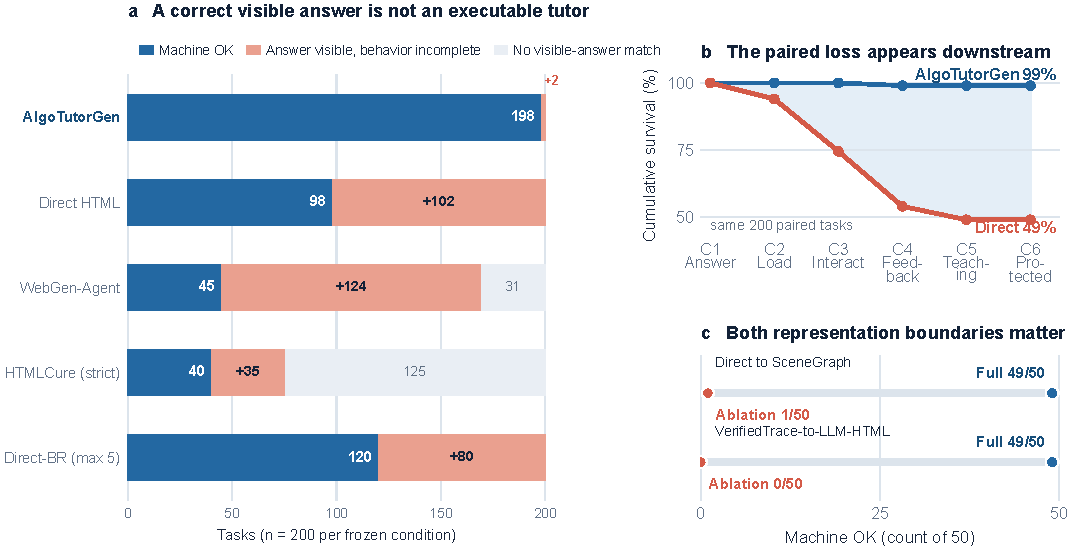
\includegraphics[width=0.96\textwidth]{figures/reliability-evidence-composite-five-methods.pdf}
\caption{Full-200 reliability and representation diagnostics moved from the main paper. (a) Frozen generation conditions are partitioned into \machineok{}, visible-answer-but-incomplete, and no-visible-answer outcomes; Direct-BR reports the adaptive best-so-far result at a maximum budget of five. Direct-BR denotes \dbr{}. (b) The primary paired \system{}--Direct comparison shows cumulative contract survival from answer visibility through protected-answer stability. (c) Two internal 50-task ablations test the executable-trace and deterministic-compilation boundaries. \htmlcure{} blocks external resources.}
\label{fig:reliability-evidence-supp}
\end{figure*}

\FloatBarrier

\section{Theory-Aligned Executable Audits}

\subsection{Representation Preservation and Determinism}

The preservation audit compares the normalized algorithm-state projection stored in each trace event, scene frame, and reachable runtime frame. The projection includes stable identifiers, values, marks, pointers, graph edges, container contents, current step, and final answer; layout, CSS, and teaching text are excluded.

\begin{table*}[t]
\centering
\small
\begin{tabular}{@{}lrrp{0.225\textwidth}p{0.245\textwidth}@{}}
\toprule
Set & Artifacts/pages & Frames/sequences & Primary use & Provenance boundary \\
\midrule
Main benchmark & 200 & 9,421 frames & Reliability, preservation, mutation & One sample per task across 23 families; selected-final artifacts \\
Held-out generation & 39 valid of 40 & -- & Frozen-task generalization & Original result remains 39/40 \\
Completed held-out audit & 40 & 4,568 frames & Semantic/state audits & Fortieth artifact is a documented targeted retry \\
Long-trace & 54 & 41,119 frames & Preservation and scalability & 18 tasks at small, medium, and large scales \\
Noninterference & 240 pages & 24,000 sequences & Browser state isolation & Main 200 plus completed held-out 40 \\
\bottomrule
\end{tabular}
\caption{Artifact sets used by the main and theory-aligned evaluations. The primary preservation row reuses the same selected-final pages as the main evaluation; the held-out and long-trace rows use the same instrumentation, compiler, and runtime. The completed held-out audit set contains one documented targeted retry that is not counted as an original generation pass.}
\label{tab:artifact-sets}
\end{table*}

\begin{table*}[t]
\centering
\small
\begin{tabular}{@{}lrrrrrr@{}}
\toprule
Method & C1 & C2 & C3 & C4 & C5 & C6 \\
\midrule
\system{} main & 100.0 & 100.0 & 100.0 & 99.0 & 99.0 & 99.0 \\
Direct HTML main & 100.0 & 94.0 & 74.5 & 54.0 & 49.0 & 49.0 \\
\addlinespace
\system{} Flash final & 100.0 & 100.0 & 100.0 & 100.0 & 100.0 & 100.0 \\
Direct Flash & 99.0 & 95.0 & 81.0 & 65.5 & 59.0 & 59.0 \\
\system{} GLM final & 99.0 & 99.0 & 99.0 & 98.0 & 98.0 & 98.0 \\
Direct GLM & 100.0 & 91.0 & 53.0 & 38.0 & 17.5 & 17.5 \\
\system{} Kimi final & 97.5 & 97.5 & 97.5 & 97.0 & 97.0 & 97.0 \\
Direct Kimi & 99.5 & 95.0 & 68.0 & 52.5 & 43.5 & 43.5 \\
\bottomrule
\end{tabular}
\caption{Cumulative nested-contract survival (percent). Cross-model \system{} rows use final-quality artifacts with recorded retries. The main paired comparison uses one frozen selected-final page per task; token-matched reliability appears in Table~\ref{tab:generation-cost}.}
\label{tab:nested-survival}
\end{table*}
\FloatBarrier

\begin{coltable}
\small
\begin{tabular}{@{}lrr@{}}
\toprule
Set & Artifact pass & Equivalent frames \\
\midrule
Main & 200/200 & 9,421/9,421 \\
Completed held-out & 40/40 & 4,568/4,568 \\
Long-trace & 54/54 & 41,119/41,119 \\
\midrule
Total & 294/294 & 55,108/55,108 \\
\bottomrule
\end{tabular}
\captionof{table}{Trace--scene--runtime projection audit.}
\label{tab:projection-audit}
\end{coltable}

Twenty stratified artifacts were recompiled and rerendered ten times each. Every artifact produced one canonical projection hash and one render hash across reruns. These observations establish representation-level agreement and tested-environment stability; independent oracle and human audits evaluate source-to-trace validity.

\subsection{Semantic Mutation and Overlay Isolation}

The mutation suite distinguishes changes that must be rejected from transformations that should be accepted. Ambiguous event deletions are not automatically classified as semantic faults because a deleted explanation or repeated mark may be redundant. Reordered unordered-set results are compared with a case-aware equivalence relation.

\begin{coltable}
\small
\begin{tabular}{@{}lrr@{}}
\toprule
Class & Expected & Observed \\
\midrule
Semantic violations & Reject & 2,198/2,198 \\
Teaching-text rewrites & Accept & 195/195 \\
Visual-metadata changes & Accept & 195/195 \\
Equivalent reorderings & Accept & 2/2 \\
\midrule
Preserving total & Accept & 392/392 \\
\bottomrule
\end{tabular}
\captionof{table}{Contract discrimination on the defined mutation suite.}
\label{tab:mutation-audit}
\end{coltable}

\begin{coltable}
\small
\begin{tabular*}{\columnwidth}{@{\extracolsep{\fill}}lr@{}}
\toprule
Condition & Outcome \\
\midrule
Four legal overlay variants & 372/372 each \\
Illegal \texttt{final\_answer}/\texttt{state} fields & 372/372 sanitized \\
Negative step & 372/372 rejected \\
Nonexistent step & 372/372 warned \\
Cross-model GLM overlay & 369/369 \\
\bottomrule
\end{tabular*}
\captionof{table}{Teaching-overlay isolation. Outcomes preserve the canonical algorithm-state hash unless marked as rejected or warned.}
\label{tab:overlay-audit}
\end{coltable}

The legal variants are original, concise, detailed, and random text overlays; their text changes do not redefine algorithm state. The existing sanitizer removes the tested protected writes, the schema rejects negative indices, and step-not-found warnings prevent unbound teaching steps. For the GLM overlay, 169 cases apply fully and 200 apply partially because model-specific traces expose different step sets. The illegal-field result is specifically sanitization rather than schema-level \texttt{extra=forbid}. Together, these tests measure discrimination across the defined mutation and preserving suites.

\subsection{Pedagogical Noninterference Stress Test}

\begin{coltable}
\small
\begin{tabular}{@{}lr@{}}
\toprule
Quantity & Count \\
\midrule
Unique pages & 240 \\
Random action sequences & 24,000 \\
Total actions & 1,561,298 \\
Pure pedagogical actions & 435,859 \\
Navigation/variant actions & 1,125,439 \\
Pages passed & 240/240 \\
Overlay artifacts passed & 240/240 \\
Observed violations & 0 \\
\bottomrule
\end{tabular}
\captionof{table}{Browser noninterference stress-test coverage.}
\label{tab:noninterference}
\end{coltable}

Pure actions are correct submission, wrong submission, hint, show answer, and clear learning log. Navigation actions are next, previous, timeline selection, reset, and variant selection. Each page receives 100 random sequences of 30--100 actions. Pure actions must preserve artifact, state, and step hashes; navigation must preserve the artifact and select the expected verified frame. No sequence produces a noninterference counterexample under this action grammar.

\section{Local Resume Versus Global Restart}

Both policies use the same structured output space, validators, and maximum of three policy decisions. Local keeps the current solution specification, repairs it, then reruns materialization and teaching. Global discards the specification and independently regenerates it before rerunning the same downstream work.

\begin{coltable}
\small
\setlength{\tabcolsep}{2pt}
\textit{A. End-to-end outcomes}\par
\begin{tabular*}{\columnwidth}{@{\extracolsep{\fill}}llrrrrr@{}}
\toprule
Model & Policy & Succ. & Calls & Tokens & Time & $p$ \\
\midrule
Flash & \localresume{} & 38/50 & 6.63 & 71,369 & 172.9 s & \multirow{2}{*}{0.4545} \\
Flash & \globalrestart{} & 42/50 & 5.50 & 62,256 & 194.2 s & \\
GLM & \localresume{} & 42/50 & 6.69 & 92,385 & 533.8 s & \multirow{2}{*}{1.0000} \\
GLM & \globalrestart{} & 43/50 & 6.65 & 96,186 & 558.2 s & \\
\bottomrule
\end{tabular*}

\smallskip
\textit{B. Paired success counts}\par
\begin{tabular*}{\columnwidth}{@{\extracolsep{\fill}}lrrrr@{}}
\toprule
Model & Both & Local only & Global only & Neither \\
\midrule
Flash & 32 & 6 & 10 & 2 \\
GLM & 37 & 5 & 6 & 2 \\
\bottomrule
\end{tabular*}

\smallskip
\textit{C. Token decomposition per successful page}\par
\begin{tabular*}{\columnwidth}{@{\extracolsep{\fill}}llrrr@{}}
\toprule
Model & Policy & Spec/repair & Teaching & Total \\
\midrule
Flash & \localresume{} & 25,031 & 46,338 & 71,369 \\
Flash & \globalrestart{} & 25,781 & 36,476 & 62,256 \\
GLM & \localresume{} & 37,342 & 55,043 & 92,385 \\
GLM & \globalrestart{} & 47,462 & 48,724 & 96,186 \\
\bottomrule
\end{tabular*}
\captionof{table}{Recovery outcomes, paired success counts, and token decomposition. Calls and tokens are per successful page and include final-failure costs; time is time-to-valid on successful cases.}
\label{tab:recovery-full}
\label{tab:recovery-pairs}
\label{tab:recovery-cost}
\end{coltable}

Flash favors Global numerically in success and tokens per success. GLM gives Local slightly lower token and time cost but one fewer success. Neither paired success difference is significant under the current rematerializing implementation, which differs from the theorem's fully checkpointed regime.

\section{Additional Reliability Evidence}

\subsection{Held-Out Tasks and Full-Sample Replay}

\begin{coltable}
\small
\begin{tabular}{@{}lrr@{}}
\toprule
Set & \system{} & Direct \\
\midrule
Held-out generation & 39/40 & 40/40 \\
Held-out \machineok{} & 39/40 & 18/40 \\
Held-out self-contained & 40/40 & 40/40 \\
\bottomrule
\end{tabular}
\captionof{table}{Additional task/input robustness.}
\label{tab:additional-robustness}
\end{coltable}

The held-out set contains 40 new cases from 15 families. The \machineok{} difference is +52.5 percentage points (95\% paired-bootstrap CI [37.5, 67.5], exact McNemar $p=9.54\times10^{-7}$). The targeted retry used to complete the semantic audit does not retroactively change 39/40 generation.

\subsection{Non-Degenerate Ablations and Browser Repair}

\begin{coltable}
\small
\begin{tabular*}{\columnwidth}{@{\extracolsep{\fill}}lrr@{}}
\toprule
Condition & Full & Ablation \\
\midrule
Direct-to-SceneGraph & 49/50 & 1/50 \\
\vtllm{} & 49/50 & 0/50 \\
\bottomrule
\end{tabular*}
\captionof{table}{Non-degenerate 50-task ablations. Both outputs are self-contained under the corrected resource parser.}
\label{tab:ablations}
\end{coltable}

Direct-to-SceneGraph isolates the fixed runtime without an executable trace and validation; its 96-point difference has a 95\% CI of [90, 100] and exact McNemar $p=7.11\times10^{-15}$. \vtllm{} isolates unconstrained page generation after a verified trace: its visible answer is 50/50, but interaction reachability and \machineok{} are 0/50. On these 50-task ablations, neither a fixed renderer nor a verified trace followed by unconstrained page generation reproduces the full-chain reliability.

\begin{table*}[t]
\centering
\scriptsize
\setlength{\tabcolsep}{5pt}
\begin{tabular}{@{}rrrrrrr@{}}
\toprule
Max repairs & \machineok{} & $\Delta$ from start & Repair calls & Repairs/task & Repair tokens/task & Cum. latency/task \\
\midrule
0 & 106/200 (53.0\%) & 0 & 0 & 0.000 & 0 & 0.0 s \\
1 & 118/200 (59.0\%) & +12 & 94 & 0.470 & 16,405 & 94.1 s \\
2 & 119/200 (59.5\%) & +13 & 176 & 0.880 & 31,379 & 177.1 s \\
3 & 120/200 (60.0\%) & +14 & 257 & 1.285 & 46,650 & 259.1 s \\
5 & 120/200 (60.0\%) & +14 & 417 & 2.085 & 78,237 & 424.8 s \\
\bottomrule
\end{tabular}
\caption{\dbr{} budget sweep. A budget of \(r\) permits at most \(r\) repairs beyond the frozen initial page. Each task stops on \machineok{} and otherwise publishes the best-so-far page. Tokens include only new repair calls. The latency column is the mean cumulative API repair latency per task, averaged over all 200 tasks.}
\label{tab:repair-budget}
\end{table*}

\begin{table*}[t]
\centering
\scriptsize
\setlength{\tabcolsep}{3.1pt}
\begin{tabular}{@{}rrrrrrrrrrr@{}}
\toprule
Budget & Load & Answer & Interact & Correct FB & Wrong FB & Hint & Show & Log & Protected & \machineok{} \\
\midrule
0 & 186/200 & 200/200 & 155/200 & 128/200 & 133/200 & 137/200 & 138/200 & 143/200 & 155/200 & 106/200 \\
1 & 200/200 & 200/200 & 165/200 & 139/200 & 144/200 & 151/200 & 151/200 & 157/200 & 165/200 & 118/200 \\
2 & 200/200 & 200/200 & 166/200 & 140/200 & 145/200 & 152/200 & 153/200 & 158/200 & 166/200 & 119/200 \\
3 & 200/200 & 200/200 & 166/200 & 140/200 & 146/200 & 152/200 & 153/200 & 158/200 & 166/200 & 120/200 \\
5 & 200/200 & 200/200 & 166/200 & 140/200 & 146/200 & 152/200 & 153/200 & 158/200 & 166/200 & 120/200 \\
\bottomrule
\end{tabular}
\caption{Nine-check outcomes under each maximum repair budget. FB denotes feedback. ``Protected'' is the browser audit's protected-state check, not the stronger randomized noninterference suite.}
\label{tab:repair-budget-checks}
\end{table*}

All 200 tasks reuse the same hash-verified frozen initial pages; none is regenerated. Each failed page is audited in Playwright, and the model receives generic browser observations plus the complete previous HTML, but not the hidden nine-field audit outcomes. The policy stops immediately after \machineok{} and otherwise selects the historical page with the most passing checks, breaking ties toward the earlier page. The budget sweep therefore evaluates nested adaptive policies rather than forced final rewrites.

The pass curve is \(106\!\rightarrow\!118\!\rightarrow\!119\!\rightarrow\!120\!\rightarrow\!120\). Relative to budget zero, exact paired McNemar \(p\)-values are 0.000488, 0.000244, and 0.000122 for budgets one, two, and three/five, respectively; these are cumulative within-task comparisons, not independent samples. The Wilson 95\% interval moves from [46.1, 59.8]\% at budget zero to [53.1, 66.5]\% at budgets three and five. The first repair recovers 12 tasks, the second and third recover one each, and the fourth and fifth recover none. Across 417 repair calls, page-level fail-to-pass occurs 14 times and pass-to-fail zero times because successful pages stop.

The 417 repairs use 15,647,489 tokens (6,998,333 input and 8,649,156 output). The concurrent sweep completes in 3,714 seconds of elapsed wall-clock time. All prompts contain the complete previous HTML. These data show a real but saturating benefit from whole-page browser repair under this frozen policy.

All reliability, qualitative, VLM, and human-calibration results reported for \dbr{} use the final best-so-far pages selected by the same adaptive max-five policy.

\section{Qualitative Results and Case Studies}

\begin{figure*}[t]
\centering
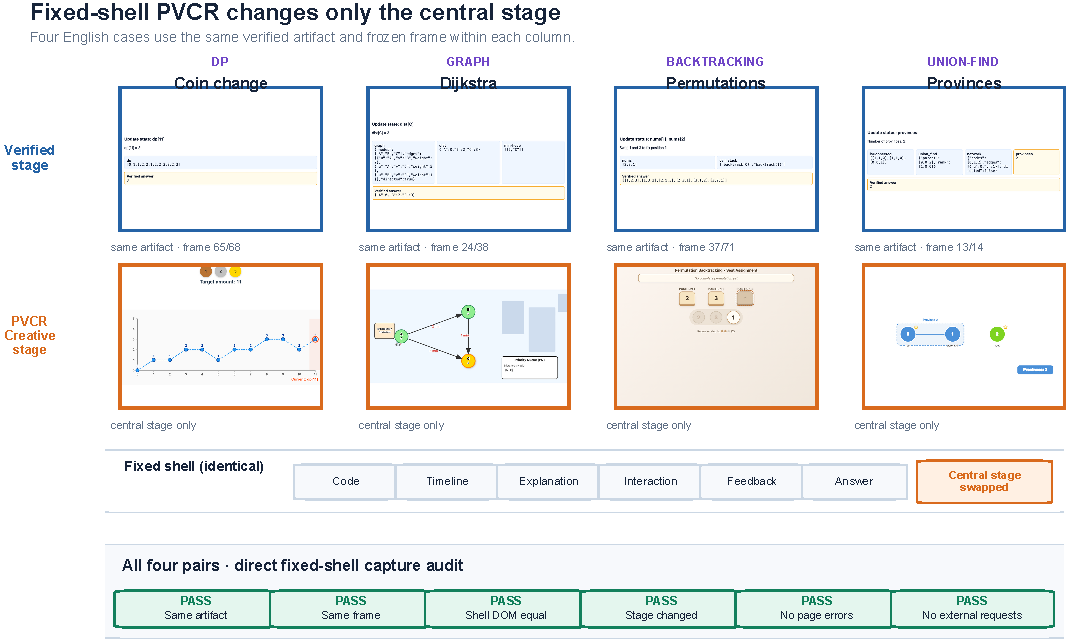
\includegraphics[width=\textwidth]{figures/pvcr-fixed-shell-four-case-gallery.pdf}
\caption{Same-artifact, same-frame central-stage crops for dynamic programming, shortest path, backtracking, and union--find. Within each column, the Verified View uses the deterministic fallback and the Creative View uses the stage-only \pvcr{} renderer. The fixed-shell capture audit verifies the same artifact, same frame, identical normalized shell DOM, a changed central stage, no page errors, and no external requests for all four pairs.}
\label{fig:pvcr-fixed-shell-gallery}
\end{figure*}

\begin{figure*}[t]
\centering
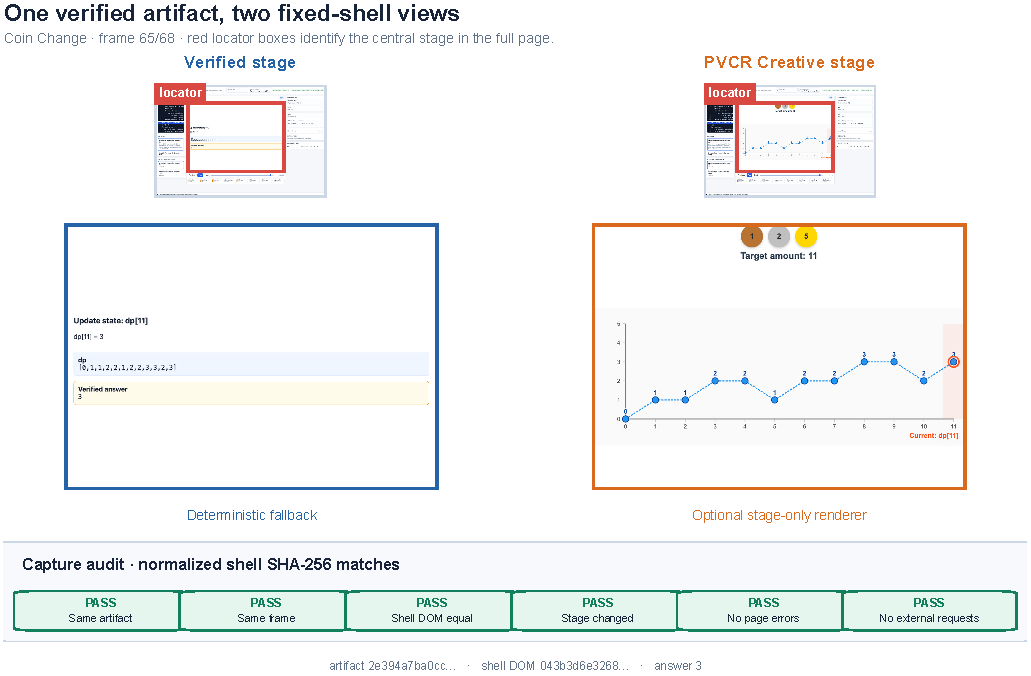
\includegraphics[width=\textwidth]{figures/pvcr-fixed-shell-pair-detail.pdf}
\caption{Detailed fixed-shell \pvcr{} pair for the English Coin Change artifact at frame 65/68. Red locator boxes identify the central stage within the two full-page captures; the enlarged crops show the deterministic Verified stage and the stage-only \pvcr{} rendering. The capture audit verifies the same artifact and frame, identical normalized shell DOM outside the stage, a changed stage, no page errors, and no external requests.}
\label{fig:pvcr-pair-detail}
\end{figure*}

\begin{figure*}[t]
\centering
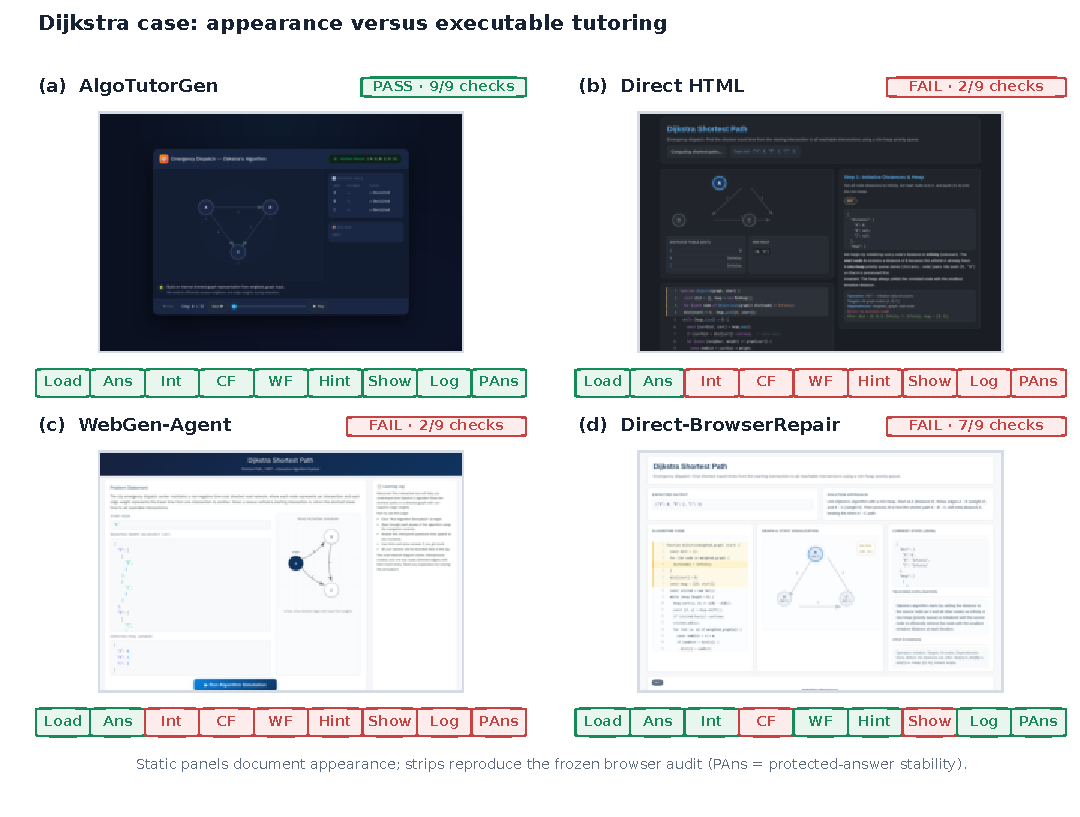
\includegraphics[width=\textwidth]{figures/qualitative_dijkstra_comparison.pdf}
\caption{A frozen Dijkstra case with a visible answer but different tutor behavior. (a) \system{} frame 24/38 shows a submitted prediction and correct feedback on the same page as the verified state and learning record. (b) Direct HTML exposes the expected answer before learner action, but static visibility does not establish the audited teaching loop. (c) \dbr{} reaches a checkpoint and records wrong feedback, while its correct-feedback and answer-reveal checks fail. (d) All five methods expose the expected answer, but only \system{} satisfies all nine contracts; Direct HTML, WebGen-Agent, and \htmlcure{} pass 2/9, whereas \dbr{} passes 7/9.}
\label{fig:dijkstra-comparison}
\end{figure*}

The figures in this section use a separate 23-case English qualitative package. Each case contains a saved \ssv{} Verified View with its page, screenshot, audit, and structured artifact JSON, together with frozen comparison pages. For the fixed-shell evidence, we re-export the available stage-only \pvcr{} asset against the corresponding saved English artifact and capture both views from one browser page at one frame. The Verified capture disables only the central-stage renderer, whereas the Creative capture restores it. The capture audit checks the same artifact and frame, equality of the normalized shell DOM outside the stage, a changed stage DOM, no page errors, and no external requests. Figure~\ref{fig:pvcr-pair-detail} shows the fixed-shell comparison in detail, while Figure~\ref{fig:dijkstra-comparison} separately compares one Verified View with four baselines.

\FloatBarrier
\clearpage

\section{Model-Token Cost and Reliability}

\noindent\begin{minipage}{\columnwidth}
At the operational all-attempt point, \system{} uses 84,352.785 tokens
per task and passes 198/200 pages, while the closest realized-cost
\dbr{} replay uses 84,254.445 tokens per task and passes 120/200. The
paired difference is +39.0 percentage points (95\% paired-bootstrap CI
[32.0, 46.0], exact McNemar $p=1.41\times10^{-21}$). Matching the
selected-final cost gives the same 198/200 versus 120/200 result, and
the maximum observed \dbr{} policy remains at 120/200 while using
97,914.885 tokens per task. Thus, under the frozen whole-page repair
policy, matching model-token cost does not close the observed
reliability gap; this comparison does not isolate the causal
contribution of individual system components.

\begin{center}
\scriptsize
\setlength{\tabcolsep}{2.5pt}
\begin{tabular}{@{}p{0.47\columnwidth}rrr@{}}
\toprule
Condition & Calls/task & Tokens/task & \machineok{} \\
\midrule
\dbr{}, no repair & 1.000 & 19,677 & 106/200 \\
\system{} selected-final & 5.330 & 76,847 & 198/200 \\
\dbr{}, selected-final matched & 2.575 & 76,854 & 120/200 \\
\system{} operational all-attempt & 5.755 & 84,353 & 198/200 \\
\dbr{}, all-attempt matched & 2.760 & 84,254 & 120/200 \\
\dbr{}, maximum observed & 3.085 & 97,915 & 120/200 \\
\bottomrule
\end{tabular}
\captionof{table}{Total model-token cost and reliability. Direct-repair totals include the frozen initial page and all included repair calls. No stable price configuration was frozen, so monetary cost is not reported.}
\label{tab:generation-cost}
\label{tab:total-token-cost-reliability}
\end{center}

\end{minipage}

\section{Long-Trace Scalability}

All 54 artifacts materialize, while 52 complete browser measurement. The exporter currently embeds complete frames in a self-contained document, so repeated state dominates size and load cost.

\begin{coltable}
\small
\setlength{\tabcolsep}{2pt}
\begin{tabular}{@{}lrrrrr@{}}
\toprule
Scale & Frames & HTML & Load & Step & Peak heap \\
\midrule
Small & 104.4 & 1.40 MB & 120 ms & 14.7 ms & 6.3 MB \\
Medium & 543.3 & 23.25 MB & 1,933 ms & 45.4 ms & 59.1 MB \\
Large & 1,636.7 & 160.42 MB & 8,354 ms & 101.3 ms & 185.6 MB \\
\bottomrule
\end{tabular}
\captionof{table}{Long-trace browser costs; all entries are means.}
\label{tab:scalability}
\end{coltable}

The large KMP page contains 3,063 frames and 581 MB of HTML. The large sliding-window-unique page contains 5,533 frames and 1.08 GB of HTML. Both exceed the 60-second load budget. These results motivate event deltas, frame virtualization, lazy loading, or state compression when scaling beyond the evaluated regime.

\section{Failure Analysis}

\subsection{Selected-Final Browser Failures}

The main \system{} condition generates valid artifacts for all 200 tasks, but two pages fail the final conjunction. \path{stack_valid_parentheses_full_core} fails wrong-answer feedback; \path{string_longest_common_prefix_full_core} fails both correct- and wrong-answer feedback. Both pages pass load, visible answer, reachable interaction, hint, answer reveal, learning log, and protected-answer stability. The first failing boundary is therefore the teaching-feedback contract, not solver materialization or scene compilation.

The final cross-model failures separate missing artifacts from generated pages with incomplete feedback. Flash has no final failure. GLM fails to generate valid artifacts for two tasks and has two generated pages with bidirectional-feedback failure. Kimi fails to generate five artifacts and has one generated page with bidirectional-feedback failure. The held-out failure is a materialization/generation failure; its missing page consequently fails all downstream browser checks. These categories are not merged into one generic ``page failure.''

\subsection{Baseline Failure Mechanisms}

Direct HTML has 12 load failures caused by JavaScript syntax, duplicate declarations, invalid escapes, or null-DOM operations. Among accepted \htmlcure{} rewrites, 125 introduce a Google Fonts request and therefore fail the strict self-contained condition when external requests are blocked. WebGen-Agent has one rendering timeout. The Dijkstra case in Figure~\ref{fig:dijkstra-comparison} was selected because every page loads and shows the answer, localizing the contrast to interaction and teaching behavior rather than a trivial parse failure.

\section{Secondary Visual Evaluation}

The formal visual comparison uses the 200 frozen selected-final pages for each of five methods. The \system{} column is explicitly the \pvcr{} Creative View generated from 200 \ssv{} Verified Views rather than the deterministic Verified View. Scores come from the same screenshot rubric and the frozen \path{output/experiments/all_method_auxiliary_eval_20260718/all_method_auxiliary_eval_report.json} report summarized in the detailed result ledger. One WebGen-Agent render failure is assigned the minimum score; the other 999 pages are VLM-scored. Correctness and release use the separate executable audits.

\begin{coltable}
\scriptsize
\setlength{\tabcolsep}{2pt}
\begin{tabular}{@{}lrrrrrr@{}}
\toprule
Method & Overall & Alignment & State & Process & Instruction & All $\geq3$ \\
\midrule
\pvcr{} & \textbf{4.755} & \textbf{4.640} & 4.670 & \textbf{4.915} & \textbf{4.795} & \textbf{199/200} \\
Direct & 4.561 & 4.455 & 4.605 & 4.660 & 4.525 & 186/200 \\
WebGen & 4.441 & 4.500 & 4.645 & 4.150 & 4.470 & 177/200 \\
\htmlcure{} & 4.300 & 4.350 & 4.445 & 4.050 & 4.355 & 163/200 \\
\shortstack[l]{\textsc{Direct-BrowserRepair}\\\textsc{(max 5)}} & 4.670 & 4.590 & \textbf{4.725} & 4.730 & 4.635 & 191/200 \\
\bottomrule
\end{tabular}
\captionof{table}{Five-method visual evaluation under one frozen screenshot rubric. All scores are 1--5 means. ``All $\geq3$'' counts pages meeting the threshold on all four dimensions. These are single-VLM proxy ratings, not human judgments.}
\label{tab:visual}
\end{coltable}

\pvcr{} is highest on the overall, alignment, process, and instructional-design means. The following human subset independently calibrates this single-VLM proxy.

Separate \pvcr{}-only reports audit the same 200 final Creative Views rather than comparing methods. All 200 pass browser smoke and strict layout, covering 1,494 frames with zero recorded non-permitted overlaps, clipping events, or text occlusions. A stricter scene-salience stress rubric identifies 51/200 high-salience pages, while algorithm readability passes 193/200; this diagnostic targets visual emphasis beyond the release gate. \ssv{} correctness is evaluated separately.

\section{Human Calibration of Visual Evaluation}
\label{sec:human_visual_calibration}

Two reviewers from the research team independently evaluated a stratified subset of 30 tasks and five methods, yielding 150 anonymized pages. Method identities and the other reviewer's ratings were hidden until both reviewers completed scoring. Each page received a 1--5 score for problem--visual alignment, algorithm-state readability, process-change clarity, and instructional visual design. Page-level human scores are the mean of the two reviewers. The evaluated \system{} condition is the \pvcr{} Creative View; the four baselines are Direct HTML, WebGen-Agent, \htmlcure{}, and \dbr{}.

\begin{coltable}
\scriptsize
\setlength{\tabcolsep}{2pt}
\begin{tabular}{@{}lrrrrrr@{}}
\toprule
Method & Align. & State & Process & Instruction & Overall & All $\geq3$ \\
\midrule
\pvcr{} Creative View & \textbf{4.39} & \textbf{4.33} & \textbf{4.27} & \textbf{4.38} & \textbf{4.34} & \textbf{29/30} \\
Direct HTML & 3.38 & 3.22 & 3.06 & 3.18 & 3.21 & 21/30 \\
WebGen-Agent & 3.67 & 3.58 & 3.47 & 3.61 & 3.58 & 24/30 \\
\htmlcure{} & 3.54 & 3.42 & 3.29 & 3.39 & 3.41 & 23/30 \\
\shortstack[l]{\textsc{Direct-BrowserRepair}\\\textsc{(max 5)}} & 3.81 & 3.69 & 3.57 & 3.72 & 3.70 & 26/30 \\
\bottomrule
\end{tabular}
\captionof{table}{Human visual ratings on 30 tasks per method. ``All $\geq3$'' requires the averaged human score to reach 3 on every dimension.}
\label{tab:human-visual-means}
\end{coltable}

Table~\ref{tab:human-visual-means} shows that \pvcr{} has the highest human mean in all four dimensions and Overall. Its Overall advantage over the strongest baseline, \dbr{}, is 0.64 points, and 29/30 Creative Views meet the four-dimension threshold. Across methods, 123/150 pages meet this human threshold.

Inter-reviewer reliability is summarized using quadratic weighted kappa (QWK).

\begin{coltable}
\scriptsize
\setlength{\tabcolsep}{2pt}
\begin{tabular}{@{}lrrr@{}}
\toprule
Dimension & Human--VLM $\rho$ & QWK & Within 1 \\
\midrule
Alignment & 0.72 & 0.76 & 144/150 (96.0\%) \\
State readability & 0.67 & 0.72 & 142/150 (94.7\%) \\
Process clarity & 0.62 & 0.66 & 139/150 (92.7\%) \\
Instructional design & 0.65 & 0.70 & 141/150 (94.0\%) \\
Overall & \textbf{0.73} & -- & -- \\
\bottomrule
\end{tabular}
\captionof{table}{Human--VLM rank correlation and inter-reviewer reliability. Weighted $\kappa$ is quadratic; the last column counts reviewer scores differing by at most one point. Reviewer A/B Spearman correlations for the four dimensions are 0.73, 0.69, 0.64, and 0.68, respectively.}
\label{tab:human-vlm-calibration}
\end{coltable}

The averaged human Overall score correlates with VLM Overall at Spearman $\rho=0.73$; dimension-level correlations range from 0.62 to 0.72. Inter-reviewer quadratic weighted $\kappa$ ranges from 0.66 to 0.76, and 92.7--96.0\% of paired ratings differ by no more than one point. Exact reviewer agreement is 106/150 for alignment, 101/150 for state readability, 95/150 for process clarity, and 99/150 for instructional design.

For the binary decision that all four dimensions reach 3, human and VLM judgments agree on 135/150 pages (90.0\%; Cohen's $\kappa=0.656$). The confusion counts are 116 pages accepted by both, seven accepted only by humans, eight accepted only by the VLM, and 19 rejected by both. Thus humans accept 123 pages and the VLM accepts 124. Disagreements mainly involve attractive pages with weak algorithm-state detail, static screenshots that obscure transitions, dense but still usable layouts, or different emphasis on local labels versus overall teaching clarity.

\begin{coltable}
\scriptsize
\setlength{\tabcolsep}{2pt}
\begin{tabular}{@{}lrrrr@{}}
\toprule
Baseline & Ours better & Base better & Tie & Mean $\Delta$ \\
\midrule
Direct HTML & 27/30 & 1/30 & 2/30 & +1.13 \\
WebGen-Agent & 24/30 & 3/30 & 3/30 & +0.76 \\
\htmlcure{} & 26/30 & 2/30 & 2/30 & +0.93 \\
\shortstack[l]{\textsc{Direct-BrowserRepair}\\\textsc{(max 5)}} & 22/30 & 4/30 & 4/30 & +0.64 \\
\bottomrule
\end{tabular}
\captionof{table}{Paired task-level comparison using averaged human Overall scores. Human and VLM method-level winner directions agree for all four baselines.}
\label{tab:human-paired-preference}
\end{coltable}

The calibration met the criteria specified before scoring: Overall Spearman is at least 0.60; all four dimension correlations exceed 0.50 and are positive; binary threshold agreement exceeds 80\%; human and VLM winner directions agree for four of four baselines; each dimension has weighted $\kappa\geq0.60$; and more than 90\% of reviewer pairs differ by at most one point. These results support the VLM score as a scalable approximation of human visual judgment on this frozen subset. Student learning outcomes are outside the present evaluation.

\section{Reproducibility}

{\raggedright
The accompanying anonymous Code and Data Supplement includes the implementation, benchmark definitions, exact production prompts, referenced JSON reports, qualitative artifacts, and a SHA-256 manifest. The principal entry points within that artifact are:
\begin{itemize}
  \item \path{docs/EXPERIMENT_RESULTS_DETAILED.md}, which records the final reporting hierarchy, configurations, totals, and source-report paths;
  \item \path{algolab/generation/prompts/} and the dynamic prompt builders in \path{algolab/generation/};
  \item \path{artifacts/method_comparison_samples_en/manifest.json}, covering 23 cases, Verified-View artifacts, frozen comparison pages, screenshots, and audit records; and
  \item \path{latex/figure-generation/AlgoTutorGen-ssv-pvcr-artifact-showcase-editable.pptx} and \path{latex/figure-generation/figure2-system-architecture-ssv-pvcr-editable.pptx}, which provide the editable qualitative and system-architecture compositions aligned with the formal \ssv{}/\pvcr{} terminology.
\end{itemize}
\par}

Browser evaluation uses a 1365$\times$900 viewport, waits 500 ms after DOM content load, searches at most 80 timeline steps for a checkpoint, and blocks external HTTP requests in strict conditions. Paired bootstrap uses seed 20260713 with 10,000 draws; noninterference sequences use seed 20260714. The recorded browser build is Playwright Chromium 1223. Remote model versions can drift, and self-contained artifacts cannot reproduce a retired remote service exactly.

\bibliography{references}

\end{document}
